\documentclass{article}
\usepackage[preprint]{neurips_2025}
\usepackage[utf8]{inputenc}
\usepackage[T1]{fontenc}
\usepackage{hyperref,url,booktabs,amsmath,amssymb,graphicx,xcolor,microtype}
\usepackage[numbers]{natbib}

\title{Forgetting Is a Certificate:\\A Verified Developmental Lifecycle for Continual Learning}

\author{%
  Anonymous Authors\thanks{Draft v3.6 (v3.5 + far-out-of-distribution sets, a second vision substrate and a language stream for the certificate-as-score measurement), 2026-09-18. All reported numbers come from evaluation seeds (2--4) never used during development; every configuration was frozen, and thresholds switched to split-conformal calibration, before these seeds were first run; the acceptance gate, which alone was iterated on those seeds, is additionally confirmed on untouched seeds 5--7 (\S\ref{sec:gate}). Every quantitative claim is
  regenerated from raw per-seed records by \texttt{claims.py}
  (output: \texttt{results/claims.json}); Appendix~\ref{app:claims} maps each
  claim to that file. Code: \texttt{ASDplusContracts/cgrow}.}\\
  Anonymous Affiliation\\
}

\begin{document}
\maketitle

\begin{abstract}
Continual-learning methods promise not to forget; none of them can prove it.
We present a system in which retention is a \emph{checked invariant} rather
than a score: a network grown as an \textbf{organism} of frozen parts
(``organs''), each behind a finite, checkable \textbf{contract} (class anchors,
margins, and a proximity territory), routed by first-accept. Growth happens
exactly where the organism abstains; the parent is never touched; and in every
run of every experiment---twelve benchmarks across three substrates---growth
caused \textbf{exactly zero answer changes}, verified bitwise. The guarantee's
price is then engineered down through a biologically ordered lifecycle:
\emph{adolescence} (gate-verified consolidation trained purely on
contract-sampled data), learned \emph{inhibition} (vetoes trained on the
contracts' own samples), and a late-maturing prefrontal \emph{arbiter}
restricted to organs whose contracts accept the input, so that every answer of
the final system is contract-covered---measured at an uncertified fraction of
$0.0000$ across all $36$ evaluation runs. Lifecycle changes are admitted by an
acceptance gate that we audit and then confirm on seeds never used for any
decision: it admits no regression above its own stated resolution, refuses
every harmful change it can resolve, and refuses no clearly-helpful one. On
held-out evaluation seeds against deliberately strengthened baselines, the
certified organism beats same-data replay on five of twelve tasks with zero
stored samples (split-MNIST $0.893$ vs.\ replay's $0.871$) and reaches $0.835$
strict on CIFAR-100 at SimpleCIL's own ViT-B/16 backbone via contracted
prototypes ($+2.2$ over SimpleCIL-last, $-8.7$ to RanPAC); the certified
lifecycle closes the strict-guarantee gap on CIFAR-100 from $18$ points to
$4$. An unconstrained arbiter would close it to $1$, but $94\%$ of its
increment comes from answering outside its own certified territories, so we
report it as an ablation, not a result. No configuration beats a properly
trained joint model, and we retract our development-time ``beats joint''
observations. Negative results are reported with their mechanisms and, where we
found them, their laws: routing headroom bounds what any router can win;
duplicate organs buy coverage, never precision; monotone boundary edits cannot
replicate selection. We argue that auditable, refusable change---not
accuracy---is the axis on which continual learning should also be scored.
\end{abstract}

\section{Introduction}
Two recent lines of work each solved half of a problem. The first
\citep[our companion developmental study;][]{evci2020rigl,dai2018nest} showed
that in growing networks it is \emph{training, not pruning}, that destroys
what a network was born with, and that trajectories which touch fewer weights
retain more---but its retention was only ever a measurement. The second, on
\emph{interval contracts} at network interfaces, showed that a boundary inside
a network can carry a finite, checkable specification sufficient to re-derive
the module behind it without data---but closed the book on growth: on both its
substrates, verified structural growth accepted zero candidates, because
training destroys the error structure growth needs.

Each hole is the other's theorem. If parts are frozen behind contracts, the
protective mechanism of the first line (weights never touched are never
overwritten) becomes an \emph{invariant} of the second; and if growth adds a
\emph{fresh representation} behind a contract rather than anchors inside an
old one, the closure of the second line dissolves. This paper builds that
synthesis and pushes it through a full developmental lifecycle.

\textbf{Contributions.} (1)~\emph{The organism} (\S\ref{sec:organism}): frozen
contracted organs in a first-accept cascade, grown where the organism
abstains. Retention is a theorem, and it is \emph{checked, not trusted}:
bitwise, in every run, growth changes no answer. (2)~\emph{The contract as its
own negative sampler} (\S\ref{sec:organism}): every unsupervised proximity
geometry we tested saturates at the same false-accept frontier; the lever that
breaks it is supervision the organism already owns---vetoes trained on
contract-sampled positives in whitened territory coordinates against real
falsely-accepted samples. (3)~\emph{The certified lifecycle}
(\S\ref{sec:lifecycle}): adolescence (verified consolidation, trained
data-free from the contracts), and---mirroring the posterior-to-anterior
maturation of cortex \citep{gogtay2004dynamic}---a prefrontal \emph{arbiter}
over frozen parts. We measure exactly where an unconstrained arbiter's
accuracy comes from, find that much of it is bought \emph{outside} every
certified territory, and adopt the territory-respecting variant, so the final
system's every answer is contract-covered. (4)~\emph{The acceptance gate}
(\S\ref{sec:gate}): every lifecycle change is admitted by a gate combining a
data-free territory check with a paired statistical test on a real held-out
escrow; we audit it against every historical decision and confirm it on seeds
never used for any decision. (5)~\emph{The price list and its laws}
(\S\ref{sec:results}, \S\ref{sec:laws}): the guarantee ladder priced across
twelve benchmarks and two backbones, and three findings---routing headroom,
the coverage-only value of redundancy, the impossibility of replicating
selection by monotone boundary edits---shown to be one mechanism.
(6)~\emph{The failure modes} (\S\ref{sec:fails}), each with a mechanism, none
tuned away.

\section{Related work}
\textbf{Continual learning.} Regularization methods
\citep{kirkpatrick2017ewc} collapse in the single-head class-incremental
setting \citep{vandeven2019three}; replay methods
\citep{shin2017dgr,rebuffi2017icarl} work by storing data or a generator;
generative classifiers \citep{vandeven2021generative} are the strongest
exemplar-free baseline at MNIST scale. In the pretrained regime, prototype
methods dominate \citep{zhou2023simplecil,petit2023fetril,mcdonnell2023ranpac}.
Architecturally our organism descends from Expert Gate
\citep{aljundi2017expertgate} and progressive networks
\citep{rusu2016progressive}; none of these provide verified retention,
audited change events, abstention semantics, or replaceable parts, which is
the axis this paper adds. \textbf{Certified training.} Our contracts reuse the
machinery of certified robustness \citep{gowal2018ibp} pointed inward at
interfaces rather than outward at perturbations; the companion contracts study
found the two guarantees do not imply each other. \textbf{Reservoirs and
interference.} The developmental companion connects reservoir computing
\citep{jaeger2001echo,maass2002liquid} to catastrophic interference
\citep{mccloskey1989catastrophic}: sparse trajectories are implicit
weight protection. Here the protection is made structural.

\section{The organism}\label{sec:organism}
An \textbf{organ} is a small prototypical trunk with spectrally capped layers
behind a \textbf{ball contract}: per-class feature anchors with margin slack
$\tau$ and radius $\rho$, plus a learned input-space \emph{territory}---per-class
PCA subspaces (means, axes, eigenvalues, calibration scalars; prototypes, never
raw samples) with cap $\rho_{\mathrm{in}}$. An organ \emph{accepts} an input
only inside its territory and with a determined margin; accepted predictions
carry a certified robust radius by arithmetic. The \textbf{organism} is a
first-accept cascade of organs frozen at birth. Its abstention region is the
\emph{need field}: growth trains a fresh organ only on what the organism
declines, and a candidate joins only if it verifiably improves the declined
validation mass (certificate parameters are solved, never penalized).
Throughout this paper, \emph{contract-covered} means an answer produced by an
organ whose contract accepted the input---a routing property checked exactly,
distinct from the per-answer robust-radius certificate that accepted answers
carry in addition.

\textbf{Retention invariant.} Under growth, the routing prefix and every
organ's decision depend only on parameters frozen at birth, so any answered
input keeps its answer under all future growth; coverage is monotone. With
monotone \emph{tightening} (accepted sets only shrink), the invariant is
\emph{no silent drift}: an answer changes only by falling through to a later
organ at an explicit, logged event. We do not trust this: every experiment
compares answers bitwise before and after every growth event. The count,
across twelve benchmarks, three substrates, all seeds and all lifecycle
configurations, is zero.

\textbf{Learned inhibition.} The organism's failure mode is
the false accept: an organ confidently claiming classes it never saw. A
shoot-out of five unsupervised proximity geometries (centroids, per-class PCA,
a capped autoencoder, combinations, a corruption discriminator) shows they
plateau at the same false-accept frontier. The lever is supervision the
organism already owns: a contract is a data generator, so when task $B$
arrives, each old organ gains a \textbf{veto}---a small capped net trained on
contract-sampled positives \emph{in the territory's whitened coordinates}
(where $z \sim \mathcal N(0, I)$ is exactly the model the spec asserts)
against the real falsely-accepted samples, conjoined with the accept rule.
Exclusion is $0.955$--$0.986$ at $6$--$10\%$ self-loss; the raw-space version
learns ``synthetic vs.\ real'' and rejects everything (self-loss $1.000$)---a
vacuous certificate. An ablation shows scalar threshold-tightening becomes
\emph{net harmful} once vetoes exist (its self-loss releases samples that
downstream organs answer wrongly): none $0.408$, scalar $0.742$, veto-only
$0.897$, both $0.819$ on split-MNIST.

\textbf{Spatial substrate.} On a spatially embedded recurrent sheet (positions
in $[0,1]^2$, hinge wiring cost, cost-weighted pruning), organs are local
recurrent populations placed by the wiring economy; growth is
\emph{directional} (a newborn may listen to frozen predecessors; no edge ever
enters a frozen row). Lesioning organ $k$ destroys its own tasks (damage
$0.96$--$0.98$) and no earlier task (lower-triangular damage $0.000$ across
all organisms); listening carries $+8.7$ points of forward transfer on
temporal streams and its cost is visible as lesion fragility. Anatomy is
modular by measurement (within-organ weight $0.93$ vs.\ a $0.25$ null) and
\emph{replaceable}: an organ re-derived from its published contract alone, at
three architectures, agrees with the original at $0.92$--$0.93$
(swapped-spec control: $0.000$).

\section{The certified lifecycle}\label{sec:lifecycle}
Development's invariant is also its ceiling: frozen errors accumulate. Biology
answers with staged consolidation---sensory cortex first, prefrontal control
last, plastic over already-frozen parts before consolidating itself
\citep{gogtay2004dynamic}. The organism affords the same stages because every
part carries a generator.

\textbf{Adolescence.} Sample labeled data from every organ's contract, train
one consolidated organ on the pooled synthetic set, and \emph{verify}: a
usefulness floor on holdout coverage (vacuous consolidations pass every safety
check---measured), and a \emph{relative} per-class gate against the organism
being replaced on identical data (absolute floors harden with class count).
At high class counts, consolidation must be into \emph{closed-form
prototypes}: the trained-trunk variant collapses on a 100-class pool ($0.40$
raw, worse with more capacity). The consolidated organ inherits the
\emph{merged} territory (a union of PCA territories is a PCA territory), which
keeps it veto-capable---this single property turns mid-life adolescence from
harmful ($-5$ points; the unvetoable version wrongly claims $19\%$ of later
classes) to net-positive ($+6$; residual channel $4$--$5\%$). Contract
\emph{guarantees} are renegotiated freely at adolescence and certified
backward-compatible by sampling (coverage kept $1.000$, agreement
$0.93$--$1.00$); \emph{territories} cannot be re-derived from generated
data---every attempt is quietly vacuous (the renegotiated organ answers
$0$--$7\%$ of real inputs and the organism silently reverts).

\textbf{The prefrontal arbiter, and where its accuracy comes from.} A small
net reads every organ's evidence (distance, margin, territory score, accept
bit) and learns \emph{who to trust}. It answers nothing; it routes. It trains
purely on contract-sampled data and stays plastic while the parts are frozen.
Left unconstrained, it answers with its argmax organ \emph{whether or not that
organ accepted the input}, and an exact additive decomposition of its gain
over first-accept (partitions: \emph{fill} where the cascade abstained,
\emph{re-route} where it answered, \emph{drop} by $\theta$-abstention) shows
what that freedom buys. On digits the gain is genuine re-routing ($134$
corrections against $4$ regressions over five seeds), but $8.6\%$ of its
answers come from a non-accepting organ and carry $45\%$ of the advantage; on
CIFAR-ViT, where $100$ fine-grained territories are a poor guide to who should
answer, outside-territory answers are $15.6\%$ of the total and carry
\textbf{94\%} of the advantage---only $18.3\%$ of its re-routes land on an
accepting organ, its abstention threshold never binds, and it has stopped
behaving like a contracted system at all. The unconstrained arbiter is
therefore not a gateable mechanism but an \emph{uncertifiable} one
(\S\ref{sec:gate} confirms this by audit), and the lifecycle adopts the
\textbf{territory-respecting arbiter}: the same net, its choice restricted to
organs that accept, abstaining when none do. Every answer of the final system
is then contract-covered by construction---measured at exactly $0.0000$
uncertified answers across all evaluation runs---at a price \S\ref{sec:results}
states plainly: the restriction keeps $72\%$ of the unconstrained gain on
digits and $32\%$ on CIFAR-ViT, where the regime-appropriate remedy is
topological (contracted prototypes, certified by construction, match the
unconstrained arbiter's accuracy). The arbiter is consolidated last behind the
same relative gate, its answer changes audited as one logged event.

\section{The acceptance gate}\label{sec:gate}
Every lifecycle change---consolidation, arbitration, renegotiation, death---is
admitted or refused by a gate. Our original gate scored per-class accuracy on
contract samples plus the last task's real validation, and two changes walked
past it: the unconstrained arbiter (accepted $3/3$ while buying $94\%$ of its
CIFAR gain outside every territory) and a boundary renegotiation that was
quietly $-0.0045$ on real test (\S\ref{sec:laws}). Both slipped through for
one reason: \textbf{gates that score contract samples certify contract
fidelity, not real behaviour}. The repaired gate adds two checks and keeps the
original, so each verdict names what fired.

\textbf{Territory}---data-free and exact. Every answer must come from an organ
that \emph{accepted} the input: no data, no labels, no threshold. It also
repairs a representational gap: the verdict reports \texttt{certified}
separately from \texttt{accepted}, making ``beneficial but uncertified''---the
honest description of the unconstrained arbiter---sayable at all. Audited
against all $21$ historical arbiter decisions, this check refuses every one of
them, harmful and helpful alike ($1.3$--$9.8\%$ of any unconstrained arbiter's
answers are outside territory), so it is a \emph{policy}, not a detector: it
prevents the wall-robot false-accept (\S\ref{sec:fails}) as a matter of
category, at the price of every beneficial unconstrained arbiter. Detecting a
regression \emph{as such} needs real data.

\textbf{Escrow}---a paired test on real held-out data, used only by gates,
never for training. Two designs failed first and both are traps worth naming.
A fixed $0.05$ per-class floor over $100$ classes at ${\sim}60$ samples each
\emph{false-refused} a territory-clean change worth $+0.024$, because the
minimum of $100$ noisy per-class estimates falls below any small fixed slack
almost surely. Drawing the escrow from \emph{train} flattered every candidate
(a genuinely $-0.0048$ change scored $+0.0003$), because organs fit train
better than test. And capping the escrow at $N$ per class silently discarded
most of a small dataset's validation split, collapsing a decisively refusable
regression ($z=-6.86$ on the full split) to an accepted one ($z=-1.57$). The
final check uses the \emph{whole} held-out validation split, judges overall
quality by a one-sided McNemar test on discordant pairs ($z \ge -1.645$; only
discordant pairs carry information), flags a class only past a Bonferroni
correction, and keeps an unconditional hard floor at $0.25$ so a single-class
collapse---the apoptosis failure mode---stays catchable regardless of
significance. In the audit it refuses all four harmful historical arbiters and
none of the eleven helpful ones (one false refusal appears only at
full-split power, on a $+0.014$ change flagged per-class); its resolution is
reported by the gate itself (\texttt{detectable\_drop}), so it degrades by
stating its limit rather than failing silently.

\textbf{Escrow independence.} The escrow shares the validation split with the
lifecycle's own gates. Splitting validation into class-stratified halves---one
for the gates, one for the escrow---changes $2$ of $30$ evaluation-seed
verdicts, both toward \emph{more} acceptance (one $-0.015$ regression and one
$+0.005$ gain now admitted); none flips from accept to refuse, which is what
reuse-inflated acceptance would produce. The reuse is benign and the cost of
independence is power (half the escrow is ${\sim}\sqrt 2$ less), so the frozen
gate keeps the whole split.

\textbf{Disclosure and out-of-sample confirmation.} The organism and lifecycle
were frozen before evaluation seeds 2--4 ran, but the gate was not: both
escrow redesigns responded to evaluation-seed failures, so the gate's
in-sample record (zero accepted regressions over $36$ runs) required
confirmation. We froze the specification above and reran the ten CPU
benchmarks on \textbf{seeds 5--7, never used for any decision}: over $30$
fresh runs the uncertified fraction stays $0.0000$, wall-robot's harmful
arbiter is refused $3/3$ ($z=-3.35,-6.34,-7.72$), no clearly-helpful candidate
is refused, and exactly one accepted change regresses---satimage seed~$6$ at
$-0.0068$, \emph{half} the gate's stated resolution for that escrow ($0.0137$
at $n{=}723$), a validation-to-test gap no test on this data could resolve.
The out-of-sample guarantee therefore takes its precise form: \textbf{the
frozen gate admits no regression above its stated resolution, refuses every
harmful change it can resolve, and refuses no clearly-helpful one.} Across all
$102$ runs of the frozen gate now on record (evaluation, confirmation, and two
class-order permutations) the exceptions are two sub-resolution slips and one
genuine miss---letter under a permuted order, $-0.023$ at $z=-1.10$, where
validation did not show a regression that test does---so the statement holds
with a measured exception rate of one in $102$. CIFAR
confirmation seeds require growing fresh organisms and are deferred to the
GPU stage of this project.

\textbf{A lifetime budget.} Sub-resolution slips can compound over a long life
of gated events, so the gate also carries a \emph{ledger}: every accepted change
records its signed escrow delta, and a candidate that passes its own test is
refused if the cumulative delta would fall below $-0.02$. On the sleeping
organism (\S\ref{sec:daring}; a gated consolidation and a gated dream every
night, seven MLP benchmarks, evaluation seeds) the escrow check alone refuses
$25$ nights the original contract-sample gate would have judged blind, and the
ledger binds exactly where predicted and nowhere else: on the one long life
(letter, $13$ nights) accepted drift accumulates to $-0.013$ and a single dream
is refused for the budget; on every five-night life cumulative drift stays
${\approx}0$ or positive. It changes no final accuracy here---its value is on
long deployments, where accumulation is the only way a correctly-gated system
can still drift.

\section{Results}\label{sec:results}

\begin{table}[t]
\centering
\caption{Class-incremental learning, single head, no task oracle, abstention
counted as error for the organism (``strict''). Evaluation seeds 2--4;
baselines strengthened (z-scored features, doubled training, doubled-width
joint). $^{L}$ = after the \emph{certified} lifecycle (territory-respecting
arbiter, repaired gate): every answer contract-covered, zero accepted
regressions. 2--3 seeds. $^{\dagger}$Shared-speaker split; under a speaker-disjoint
split every method loses roughly half its accuracy (organism $0.35$, replay $0.45$,
joint $0.52$; \S\ref{sec:fails}).}
\label{tab:main}
\small
\begin{tabular}{lccccc}
\toprule
benchmark & fine-tune & EWC & replay & \textbf{organism} & joint \\
\midrule
split-digits (5$\times$2) & 0.58 & 0.58 & 0.93 & 0.88 (\textbf{0.91}$^{L}$) & 0.98\\
split-MNIST (5$\times$2) & 0.25 & 0.39 & 0.87 & \textbf{0.89} & 0.98\\
split-KMNIST (5$\times$2) & 0.27 & 0.34 & 0.77 & \textbf{0.81} & 0.96\\
split-Fashion (5$\times$2) & 0.21 & 0.32 & 0.78 & \textbf{0.80} & 0.89\\
letter (13$\times$2) & 0.04 & 0.10 & 0.50 & \textbf{0.78} & 0.95\\
satimage (3$\times$2) & 0.33 & 0.33 & \textbf{0.88} & 0.83 & 0.90\\
wall-robot (2$\times$2) & 0.23 & 0.36 & 0.72 & \textbf{0.80} & 0.91\\
sheet, synthetic streams & --- & --- & 0.99 & 0.98--0.99$^{L}$ & 1.00\\
sheet, spoken digits$^{\dagger}$ & --- & --- & 0.93 & 0.77 (0.79$^{L}$) & 0.95\\
CIFAR-100, frozen R18 & --- & --- & 0.59 & 0.40 (0.47$^{L}$) & 0.67\\
CIFAR-100, ViT (lifecycle) & --- & --- & 0.86 & 0.67$\to$\textbf{0.79}$^{L}$ & 0.81\\
CIFAR-100, ViT (contr.\ protos) & --- & --- & --- & \textbf{0.84} & 0.84 (NCM)\\
\bottomrule
\end{tabular}
\end{table}

\begin{table}[t]
\centering
\caption{Against published results, where standard protocols exist. All
``this work'' numbers are the certified configuration; the unconstrained
arbiter's higher numbers appear in parentheses as ablations. MNIST-scale
anchors are the class-IL benchmark runs of
\citet{vandeven2019three,vandeven2021generative} (iCaRL and DGR are their
implementations of \citet{rebuffi2017icarl} and \citet{shin2017dgr}); both
ViT-scale anchors are \emph{final} (last-step) accuracies, the same metric as
our strict score.}
\label{tab:published}
\small
\begin{tabular}{lll}
\toprule
setting & best published & \textbf{this work, certified} \\
\midrule
split-MNIST, exemplar-free & gen.\ classifier 0.938 \citep{vandeven2021generative}; DGR 0.913 \citep{shin2017dgr} & 0.893 (0.915 unconstr.)\\
split-MNIST, with buffer & iCaRL 0.946 \citep{rebuffi2017icarl} (2{,}000 exemplars) & 0.893, zero stored data\\
split-MNIST, same-data replay & strengthened replay 0.871 & \textbf{0.893}, zero stored data\\
CIFAR-100, ViT-B/16-in21k & SimpleCIL 0.813 last \citep{zhou2023simplecil}; RanPAC 0.922 \citep{mcdonnell2023ranpac} & \textbf{0.835} / 0.844 forced (protos); 0.794 lifecycle\\
CIFAR-100, DINOv2-B & no verified class-IL anchor; same-feature NCM 0.873, same-data replay 0.889 & \textbf{0.865} / 0.873 forced (protos); \textbf{0.865} lifecycle\\
CIFAR-100, ViT-L/16-in21k & no verified anchor; NCM 0.877, replay 0.892 & \textbf{0.867} / 0.877 forced (protos); 0.861 lifecycle\\
ImageNet-R, ViT-B/16-in21k & SimpleCIL 0.546; APER-adapter 0.680 \citep{zhou2023simplecil}; RanPAC 0.779 \citep{mcdonnell2023ranpac} & \textbf{0.524} / 0.551 forced (protos); 0.431 lifecycle\\
ImageNet-A, ViT-B/16-in21k & SimpleCIL 0.489; APER-adapter 0.494 \citep{zhou2023simplecil}; RanPAC 0.624 \citep{mcdonnell2023ranpac} & \textbf{0.454} / 0.511 forced (protos); 0.450 lifecycle\\
CUB-200, ViT-B/16-in21k & SimpleCIL 0.867; APER-adapter 0.871 \citep{zhou2023simplecil}; RanPAC 0.903 \citep{mcdonnell2023ranpac} & \textbf{0.858} / 0.866 forced (protos); 0.822 lifecycle\\
ObjectNet-200, ViT-B/16-in21k & SimpleCIL 0.536; APER-adapter 0.580 \citep{zhou2023simplecil}; RanPAC not reported & \textbf{0.506} / 0.543 forced (protos); 0.400 lifecycle\\
OmniBenchmark, ViT-B/16-in21k & SimpleCIL 0.732; APER-adapter 0.744 \citep{zhou2023simplecil}; RanPAC 0.799 \citep{mcdonnell2023ranpac} & \textbf{0.724} / 0.733 forced (protos); 0.669 lifecycle\\
VTAB, ViT-B/16-in21k & SimpleCIL 0.844; APER-adapter 0.844 \citep{zhou2023simplecil}; RanPAC 0.922 \citep{mcdonnell2023ranpac} & \textbf{0.888} / 0.893 forced (protos); 0.886 lifecycle\\
CIFAR-100, from scratch & DER 0.653 last \citep{yan2021der}; FOSTER similar \citep{wang2022foster} (trained backbone, 2{,}000-exemplar buffers) & not comparable (frozen R18: 0.40; ceiling 0.67)\\
\bottomrule
\end{tabular}
\end{table}


\begin{figure}[t]
\centering
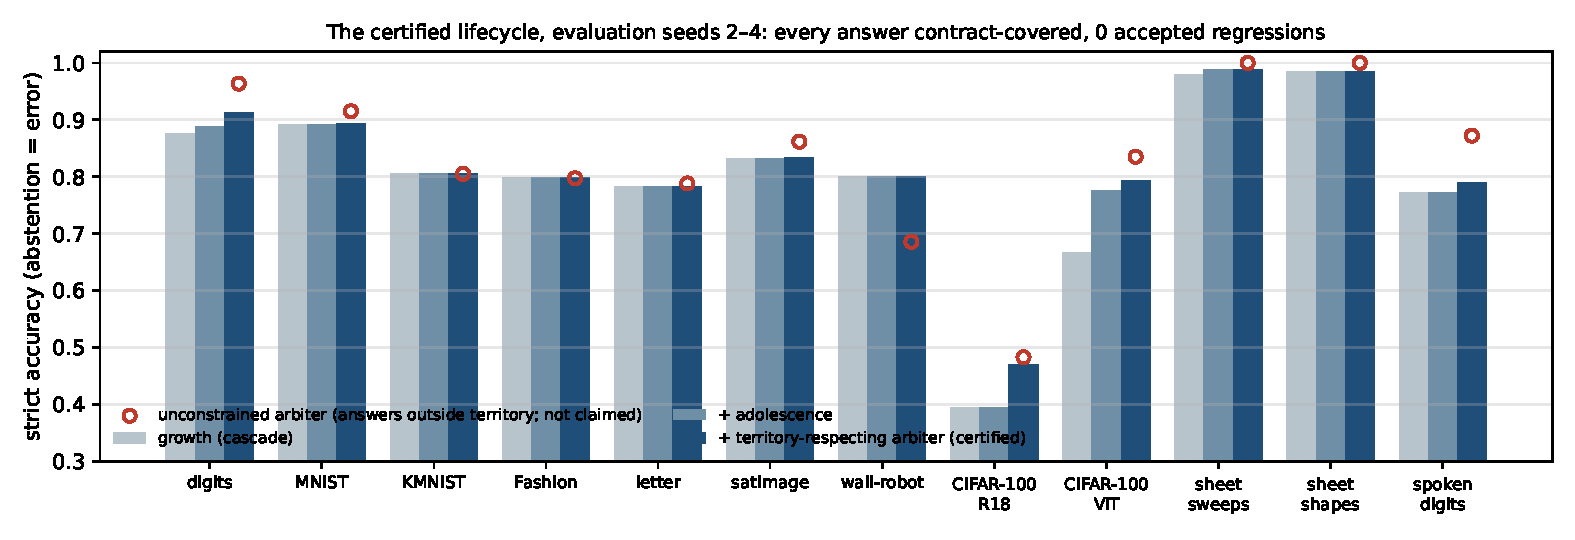
\includegraphics[width=\linewidth]{fig_lifecycle.pdf}
\caption{The certified lifecycle on all twelve benchmarks (evaluation seeds
2--4, strict accuracy): growth, adolescence, and the territory-respecting
arbiter under the repaired gate. Every bar is contract-covered; hollow markers
show the unconstrained arbiter, whose extra accuracy is bought outside
certified territory and is not claimed. Refused stages carry the previous
stage forward, which is why several bars are flat.}
\label{fig:lifecycle}
\end{figure}

\textbf{The guarantee ladder, priced.} On CIFAR-100 the same features support
three regimes: bitwise answer-stability (cascade), frozen-prototypes with
logged drift, and no guarantee. The strict guarantee costs $\approx$16 points
on weak features, about the same on strong ones ($0.667$ vs.\ $0.844$ on
evaluation seeds), and $\approx$0 on the MNIST ladder---the exchange rate is
set by how well the features separate classes. The logged-drift rung costs
nothing versus free NCM and adds a working certificate: drift is
$5$--$17\times$ more often corrective than harmful and is \emph{forecastable
before each event} from contract samples alone on the promised region
(correlation $0.65$--$0.98$, calibration $1.5$--$2\times$).

\textbf{The certified lifecycle, and what certification costs.} On CIFAR-ViT
evaluation seeds: growth $0.667 \to$ adolescence $0.776 \to$
territory-respecting arbiter $0.794$ ($3/3$ seeds, all gates passing), with
every answer contract-covered; contracted prototypes remain the strongest
fully-covered configuration at $0.835$ strict / $0.844$ forced, so our
CIFAR-ViT recommendation is the prototype topology rather than
cascade-plus-arbiter. That recommendation is substrate-dependent. On three
stronger frozen caches (ViT-B/16 on the full train set, DINOv2-B, ViT-L/16;
evaluation seeds, frozen gate) the contracted prototypes' forced accuracy
equals nearest-class-mean on the same features to the third decimal
(0.842 / 0.873 / 0.877) and the strict number trails it by the $0.8$--$1.0$
point of abstention the contract buys: the certificate rides feature quality
one-for-one but never above the prototype topology it wraps, so the $8.7$-point
gap to RanPAC on ViT-B is its trained random-projection head, not the
features. DINOv2-B gives the best certified CIFAR-100 number, $0.865$, and
there the cascade route equals the prototype route ($0.865$ vs.\ $0.865$)
because the free arbiter's headroom over the cascade has shrunk from
$+0.059$ to $+0.008$; the gate refuses the arbiter in $8$ of $9$ runs, each
time by the last-task validation clause, forgoing $+0.001$ to $+0.007$,
and accepts one change of $+0.001$, so its record stays at zero accepted
regressions over $45$ evaluation runs. Same-data replay still leads by
$2.5$--$3$ points on every backbone. On the six-dataset pretrained-model suite those papers
report on with the same backbone (ImageNet-R, ImageNet-A, CUB, ObjectNet,
OmniBenchmark, VTAB; features extracted on a GPU, pipeline unchanged, seeds
2--4) the finding repeats without exception: forced equals nearest-class-mean
to the third decimal on all $18$ seeds and lands within about one point of
SimpleCIL's last-step accuracy on five datasets (Zhou et al.'s supplementary
Inc20/Inc30 tables, IN21K block), while RanPAC's head buys a further $4$--$23$
points. The certified lifecycle trails the prototypes by $0.2$--$10.6$ points in
proportion to how much of the input the consolidated organ answers (91--100\%
on VTAB, ImageNet-A, CUB; 43--75\% on ImageNet-R, ObjectNet, OmniBenchmark),
and the gate refused all $18$ arbiter proposals, $11$ of them on the escrow's
real-data test. The suite also exposed three latent defects in code that had
only ever seen full-width territories (a shape error for classes with fewer
than 25 samples; NaN anchors and NaN-poisoned gate aggregates for classes with
almost no data), fixed without touching any threshold and with no effect on
any earlier number. We also correct one anchor: the CIFAR-100 APER-adapter
value we quoted earlier ($0.852$) was the B0 Inc5 column; at B0 Inc10 it is
$0.875$. Finally, two curricula in the developmental sense (a different
protocol, compared only to the random-order lifecycle of the same seeds) locate
where scaffolding matters. Contracted prototypes are order-invariant by
construction; only the cascade moves. Ordering CIFAR-100 tasks by superclass
(confusable classes together) raises growth from $0.667$ to
$0.698$ and the certified lifecycle from $0.794$ to
$0.799$, while easy-first, hard-first and spread orders stay within the order
band. Growing 20 superclass \emph{containers} first and refining each with a
child organ inside its territory reaches $0.626$ fine strict
($0.696$ forced) with 30 vetoes instead of
250, zero fine-level flips across ten refinements, and a certified
coarse answer on 20\% of inputs; but it cannot reach the flat
prototypes, because a 20-way nearest-mean over superclasses scores $0.849$ on
these features against $0.911$ for the fine means mapped to superclasses, a
loss no refinement recovers (hierarchical NCM ceiling $0.777$ vs.\ $0.843$).
Scaffolding pays in inhibition, stability and graded answers, not in accuracy;
the unit that helps accuracy is task composition, not a coarse label. Prototype children (closed-form anchors, no trunk) leave fine accuracy essentially unchanged (0.665 vs.\ 0.626) at a fraction of the parameters; two-step refinement inside containers needs 138 within-container vetoes and produces no within-container flips; and consolidating progressively every two tasks ends at 0.771 against 0.776 for one consolidation at the end, with every proposal gated. The lever itself was then measured: a RanPAC-style random-projection ridge
head placed under the same contract (per-class PCA territory, margin on the
head's top-two scores) moves certified strict accuracy on CIFAR-ViT from
$0.835$ to $0.875$ and on DINOv2-B from $0.865$ to $0.901$,
within a point of RanPAC's head-only row on CIFAR and level with its full result
on VTAB ($0.929$), while coverage stays above $0.96$ everywhere but
ImageNet-A, where a second-order head has too few samples per class and the
contract refuses accordingly. What the head gives up is the cascade's
invariant: already-given test answers change 8--155 times per 100
test points over a run because the ridge weights are re-solved, against exactly
zero for the cascade; the contract restores coverage semantics but not retention. We then tested whether the two can be had at once. Freezing the head the
way an organ is frozen -- one ridge block per task, solved from that task's rows
alone and never re-solved, answers taken first-accept in birth order -- delivers
the invariant exactly: appending a block changes zero answers, checked bitwise on
every seed. It does not deliver the accuracy. Against the re-solved head it loses
$38.7$ points on CIFAR-100 ($0.482$ vs.\ $0.869$), $20.5$ on DINOv2-B and $54.1$ on VTAB, falling below even the contracted prototypes. The reason is structural rather
than an implementation gap: a ridge readout's advantage over class means is that
it is solved over all classes jointly, and a block frozen at birth has no
negatives for classes that do not yet exist. Retention requires the answer to be
fixed when first given; joint decorrelation requires knowing every class. We
therefore report accuracy and bitwise retention as separate configurations, with
the reason named. Three further measurements price the configurations (\S\ref{sec:gate} protocol, seeds 2--4). Cutting the same CIFAR-100 stream into 20, 50 and 100 updates leaves the prototypes' answers identical to twelve decimals and the cascade's growth flips at zero over 501 checked steps, while the re-solved head ends at the same accuracy and rewrites $13\to41$ answers per 100 test points along the way ($40\to141$ on ImageNet-R); the certified lifecycle falls from $0.795$ to $0.729$ at 100 organs, and the escrow refused a candidate $14$ points worse than its incumbent on every seed there. As an out-of-distribution score the certificate slack ranks CIFAR-10 against CIFAR-100 at AUROC $0.841$, textures (DTD) at $0.995$ and out-of-scope text against CLINC150 intents at $0.955$ -- above kNN, NCM-cosine and Mahalanobis on the same features but below a jointly trained probe's softmax -- yet at its own operating point it still accepts $79$\% of CIFAR-10 and $99$\% of SVHN digits, which a frozen encoder maps inside object territories: the certificate bounds where an answer came from, not how far outside an input lies. After the shared encoder the prototypes cost $1.9$\,M floats, the cascade $4.9$\,M, and the M$=10{,}000$ head $10.6$\,M plus a $101$\,M-float Gram to keep learning; the two configurations that never change an answer carry no learning state at all. The headline table replicates on its own untouched seeds 5--7 (all seven datasets, first-session adapters): the contracted head moves by at most $1.4$ points, growth flips are 0 on 21/21 seeds, the gate accepted 3/21 arbiters with one sub-resolution regression ($-0.4$, CUB) and no helpful refusal, and the CIFAR arbiter that was accepted 3/3 on the evaluation seeds is refused 3/3 here at the rule's threshold. On RanPAC's own checkpoint family the head with adapters reaches forced $0.777$ / $0.607$ / $0.895$ on ImageNet-R / -A / CUB against RanPAC's $0.779$ / $0.624$ / $0.903$, the remaining difference being the metric definition. The certificate transfers unchanged to a frozen sentence encoder (Banking77, CLINC150: head $0.921$ / $0.950$ strict, above same-data replay and a joint MLP, flips 0) and to raw intrusion-detection rows (NSL-KDD: head $0.935$, prototypes $0.428$ because class means do not separate that space, every consolidation refused, correctly). Finally we ran the one ingredient the published leaders have and we did
not: a single parameter-efficient tuning of the backbone on the first task,
frozen thereafter (rank-16 adapters, $0.31$M parameters against the backbone's
$86$M). Read in our terms this is a birth step, so it costs no guarantee: with
it the contracted head reaches $0.906$ on CIFAR-100 (APER-adapter $0.875$, RanPAC $0.922$), $0.763$ on ImageNet-R (APER $0.680$), $0.639$ on ObjectNet (best published APER variant $0.582$) and $0.939$ on VTAB, above RanPAC's full result there, with coverage $0.97$--$0.99$ and growth flips still exactly
zero. The exception is instructive: on OmniBenchmark the birth step \emph{lowers}
feature quality ($-0.012$ joint nearest-class-mean) and the acceptance gate then
refused the consolidation that follows it on all three seeds, so the anatomy
stayed as grown. Extracting the three datasets whose published RanPAC numbers
use the ImageNet-1K-fine-tuned checkpoint reproduces its own nearest-class-mean
ablation to within a point and closes that confound. One gate was still weaker than the rest and is now fixed. A
consolidation used to face real held-out data only on the last task, the other
classes being represented by contract samples alone; it now also faces the
escrow the arbiter gate uses, over the whole validation split and every class
seen so far. Replaying all $67$ cached organisms through the old rule and the new one shows the old gate was not being misled: none of the $57$ decisions that reach the escrow has negative overall evidence (median McNemar $z = +13.4$), so every consolidation already on record is corroborated by real data. The escrow adds exactly one refusal, where a
class falls from $24/26$ to $17/26$ validation samples: refusing costs $12.2$
points of test accuracy and protects that class, which is the trade the doctrine
asks for. Transplanting the escrow verbatim first produced three false
refusals, because its per-class hard floor was a fraction with no condition on
how many samples the breach represented; on a benchmark with $120$ classes at a
median of $14$ validation samples a three-sample swing tripped it. The floor now
requires at least five lost samples, which leaves the collapse it exists for
catchable and had never fired in the $41$ arbiter decisions on record. Against the unconstrained run, certification costs
$1$--$8$ points on eight of twelve benchmarks (spoken digits $-0.082$,
CIFAR-ViT $-0.041$, digits $-0.036$, MNIST $-0.022$, shapes $-0.015$,
CIFAR-R18 $-0.013$, satimage $-0.009$, KMNIST $-0.007$), leaves three
unchanged, and \emph{improves} wall-robot by $+0.114$, because the
unconstrained run had accepted a catastrophic arbiter there. Fifteen of $36$
arbiters are accepted, zero accepted changes regress, and the split-MNIST
scoreboard against same-data replay reads five of twelve (down from six under
the unconstrained arbiter; certified digits $0.912$ no longer clears replay's
$0.933$). Certification costs real accuracy on most benchmarks and buys it
back only where the unconstrained version was badly wrong---which is the
argument for it. Class order is not innocent: two random permutations of the
task order move the certified numbers by $0.4$--$4.8$ points on the MLP
benchmarks (most on wall-robot and Fashion, least on 13-task letter), with the
default order best on some and worst on others, so single figures on the
small-task benchmarks carry a $\pm 2$--$4$ point order band. Figure~\ref{fig:lifecycle} shows every benchmark;
Appendix~\ref{app:lifecycle} tabulates them.

\section{Three findings, one mechanism}\label{sec:laws}

\begin{figure}[t]
\centering
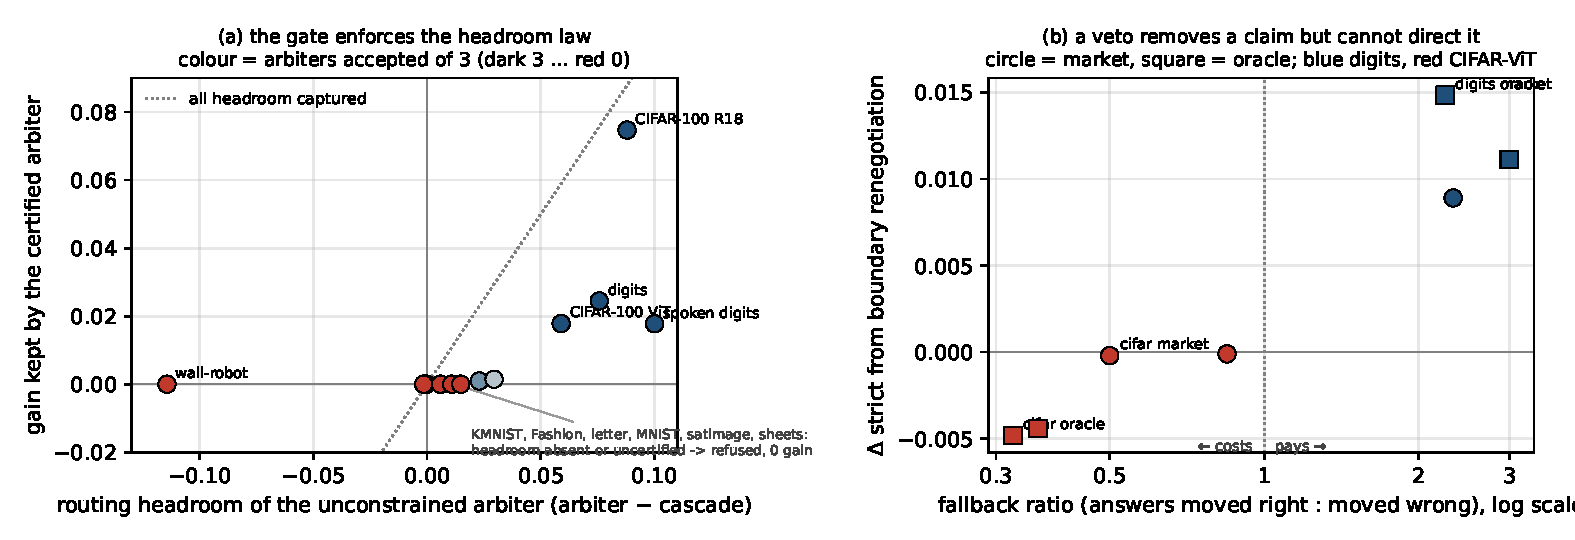
\includegraphics[width=\linewidth]{fig_laws.pdf}
\caption{Two of the three laws. (a) The gate's verdicts reproduce the
routing-headroom law without being told it: arbiters are accepted exactly
where contract-covered headroom exists (upper right), refused where headroom
is absent or negative, and refused where it exists but lives outside
territory (the cluster at zero). (b) Boundary renegotiation pays only where
the cascade's fallback is good: the fallback ratio separates the digits gains
from the CIFAR-ViT losses, and even an oracle given the labels loses on
CIFAR---a veto removes a claim but cannot direct it.}
\label{fig:laws}
\end{figure}

Three arcs of this study---redundant growth, market-based routing, and
market-based contract renegotiation---end in laws that turn out to be the same
statement seen from different sides. The acceptance gate's verdicts reproduce
all three without being told them (Figure~\ref{fig:laws}).

\textbf{Routing headroom bounds every router.} The gap
$\mathrm{arbiter}-\mathrm{cascade}$ measures what any re-routing mechanism can
win. It is benchmark-specific: $+0.001$ on KMNIST (first-accept already
\emph{is} the optimal router there, so re-routing by price can only destroy
the birth-order prior), $+0.082$ on digits, $+0.062$ on CIFAR-ViT. Where
headroom exists, a market with pool-calibrated prices takes most of it and can
tie the central arbiter ($0.836 \pm 0.002$ vs.\ $0.835 \pm 0.003$ on
consolidated CIFAR-ViT, with no central trained state); where it does not, no
pricing scheme helps. The gate enforces this unknowingly: on both evaluation
and confirmation seeds it accepts arbiters $3/3$ exactly where
\emph{contract-covered} headroom exists (digits, CIFAR-R18, CIFAR-ViT, spoken
digits), refuses where headroom is $\le 0$, and refuses where headroom exists
but lives outside territory (satimage, the sheets: the covered share is
$\le 5\%$).

\textbf{Duplicate organs buy coverage, never precision.} Growing the same
class split twice and concatenating looks like a free ensemble; it cannot be
one, because the first-accept prefix wins every contest. Measured over
$k=1\ldots4$ independent organisms (digits, five seeds): precision on covered
inputs drifts $0.929 \to 0.922$ while coverage climbs $0.934 \to 0.981$, with
zero flips against the prefix at every $k$---the entire $+0.038$ is
abstention-filling, with sharply diminishing returns (the marginal twin
answers its new inputs at $0.854$, then $0.717$, then $0.417$). Width is not a
substitute ($0.872$ at $59\%$ more parameters than the twins' $0.905$). The one
contract-covered ensembling gain on the twin pool---majority vote among
accepting organs, $+0.010$---is a \emph{null} on every grown organism ($0$
answers changed in $30$ runs across ten benchmarks, at contest rates up to
$0.84$ and up to $13$ organs): organs that co-accept an input agree on its
label, because vetoes leave only the generalist and the true specialist
accepting. Voting had something to route only where competence was
duplicated, and a grown anatomy never duplicates it.
Redundancy and the unconstrained arbiter are \emph{substitutes} (stacking adds
$+0.004 \pm 0.006$: both climb to the same ${\approx}0.96$ ceiling by
different routes), but redundancy and \emph{certified} arbitration are
\emph{complements} on digits ($0.946$ fully covered, $72\%$ of the
unconstrained gain), because redundant coverage removes exactly the channel
---filling---that certification forbids. On the flagship the complement
vanishes ($32\%$ kept) and the remedy is topological: contracted prototypes.
A by-product settles organ death: on this \emph{grown} anatomy a sound
per-class death certificate retires nobody (the anatomy is minimal), while on
a twin anatomy it retires exactly one of each pair ($5.0 \pm 0.0$ of $10$ on
KMNIST at a cost of $0.003$)---so ``no deaths'' is a fact about the anatomy,
not the gate (\S\ref{sec:daring}).

\textbf{Selection cannot be replicated by monotone boundary edits.} Since the
unconstrained arbiter's power is choosing \emph{who} answers, we asked whether
its gain could be moved inside the certificate by renegotiating the
territories themselves: organs bid pool-calibrated prices over the shared
contract pool, and whatever an organ loses is removed by a veto, so the
renegotiated contract is still a finite checkable spec. On digits this works
and the \textbf{market matches an oracle given the labels} ($+0.0148$ both,
fully certified, no inference-time trained component: what ships is a redrawn
spec). On CIFAR-ViT even the oracle \emph{loses} $0.0045$: a veto removes a
claim but cannot direct it---renegotiation is subtractive, so first-accept
hands each ceded point to the next accepter in birth order, not to the bid
winner. The \emph{fallback ratio} (answers moved right against moved wrong)
tracks the outcome monotonically across every configuration ($3.00$/$2.25$ on
digits, gains; $0.76$/$0.35$ on CIFAR, losses) and is computable on the
contract pool \emph{before} committing to any change. Two corollaries from the
pricing arc: prices need joint \emph{data} but not a central model
(self-priced routing is anti-calibrated, Brier $0.31$--$0.71$; calibrating the
same per-organ curves on the shared pool improves Brier up to $200\times$);
and the auction needs a generalist \emph{participant}, not a price
index---adding the consolidated organ as an ordinary bidder is worth $+0.09$
to $+0.16$ everywhere (a gate-refused generalist scoring $0.187$ alone still
delivers $+0.092$ as a bidder: answering and pricing are different jobs),
while indexing the reserve to its bid adds nothing.

\section{The daring program}\label{sec:daring}
Five speculative mechanisms under the same frozen protocol on evaluation
seeds: two work, one resolves into a positive claim about the anatomy, and
two fail into the laws of \S\ref{sec:laws}.

\textbf{Sleep cycles work if the organism dreams.} Nightly gated
consolidation plus a nightly arbiter rehearsal matches the one-shot lifecycle
(digits $0.950$ vs.\ $0.948$; CIFAR-ViT $0.813$ vs.\ $0.835$) while adding the
\emph{anytime} property and structural immunity to mid-life failure.
Dreamless sleep costs $4$--$6$ points: an eagerly consolidated organ
front-runs the cascade and starves new organs; the rehearsal compensates.

\textbf{Apoptosis: the leak was per-class, and a sound certificate retires
nobody.} Gated organ death with the contract archived to a \emph{genome}
(which provably still powers later consolidations) retires $7$--$9$ of $10$
organs at $4$--$8\times$ compression---but accuracy leaks $\approx 8$ points
through four escalating certificates (local synthetic, globally anchored
synthetic, real escrows of $200$ and $1{,}000$ samples; the last two
identical, so the global check never binds). A fifth certificate adds
\emph{per-class} floors on a real escrow: \textbf{zero deaths, zero leak}.
The diagnostic pins the mechanism: for a typical candidate every mean-based
gate approves (coverage kept $0.97$--$0.99$, global accuracy $+0.001$) while a
single class drops $6.7$--$13.3$ points; $19$ of $20$ refusals cite the
per-class gate. The earlier leak was real damage invisible to means; the
anatomy is minimal (no organ redundant at per-class resolution); and the twin
control of \S\ref{sec:laws} shows the certificate fires when redundancy is
real. Death is the most expensive certificate in the lifecycle, and its price
is per-class held-out data.

\textbf{The market arc} (compressed; laws in \S\ref{sec:laws}). Self-priced
decentralized routing fails by anti-calibration; a market-maker calibrating
the same per-organ curves on the shared contract pool repairs the prices and,
after consolidation, ties the central arbiter on the flagship; used at
contract-formation time it matches an oracle on digits and cannot help on
CIFAR, where selection, not boundaries, is what the cascade lacks.

\textbf{Second-order contracts: an SLA on the organism's own drift.} Before
each change event the system publishes a bound (its contract-sampled forecast
times an online conformally calibrated factor, $\alpha{=}0.25$,
preregistered). Over $54$ events: $5$ violations ($9.3\%$ against the $25\%$
budget) at median tightness $1.1$--$1.45\times$; online calibration beats the
fixed prior $5$ vs.\ $14$.

\textbf{The fractal organism composes.} A super-organ wraps a whole
sub-organism behind one merged territory (a union of PCA territories is a PCA
territory) and presents the standard organ interface, top-level vetoes
included. Ten tasks in three super-epochs: strict $0.718 \pm 0.003$,
top-level growth flips exactly $0$ (the invariant survives nesting), and an
entire $\sim$30-class super-organism re-derived from its merged contract
alone agrees at $0.75$--$0.78$ on its jurisdiction.

\section{The feature ledger}\label{sec:ledger}
Every remaining mechanism isolated through the full pipeline on both
flagships (evaluation seeds; removal rule preregistered). Nothing is removed:
vetoes are the backbone (removal: $-0.19$ MNIST, $-0.50$ CIFAR-ViT---the
arbiter does \emph{not} subsume inhibition; without vetoes growth itself
drowns at $0.10$--$0.13$), the spectral cap earns its keep ($-0.02$/$-0.07$;
uncapped evidence also breaks the arbiter gate on all six runs), and
adolescence adds $+0.09$ beyond the arbiter (consolidation repairs
representation; arbitration repairs routing). Previously measured and
excised: scalar tightening ($-0.08$ when added back), trunk-mode
consolidation, mid-life timing ($-0.05$), renegotiated territories (vacuous),
self-priced routing, the unconstrained arbiter (uncertifiable).

\section{What fails, and why}\label{sec:fails}
\textbf{Weak features break the cascade.} With 100 fine-grained classes on
frozen ResNet-18 features, territories overlap; vetoes halve rather than
erase false accepts; NCM wins ($0.55$ vs.\ $0.39$). The regime-appropriate
topology is prototypes; the contract machinery ports to it at zero cost, the
cascade does not. \textbf{Gates are certificates relative to contract
fidelity.} On wall-robot the unconstrained arbiter passed both original gate
signals yet regressed $\approx\!12$ points on test, systematically, on all
three evaluation seeds: the sampler misrepresents old tasks and contract
samples cannot see it. The repaired gate refuses it---by escrow on real data,
decisively, on evaluation and confirmation seeds alike---but the episode's
lesson stands: detecting a real-data regression requires real held-out data,
and the gate's power is bounded by the escrow it is given
(\texttt{detectable\_drop} states the bound). \textbf{The spoken-digits benchmark leaks speaker identity.} All FSDD numbers
above use the standard random split, which shares the same six speakers across
train, validation and test. Holding one speaker out for test and another for
validation, \emph{every} method collapses---organism $0.772 \to 0.349$
(certified lifecycle $0.328$), replay $0.93 \to 0.45$, the joint model
$0.95 \to 0.52$---so the collapse belongs to the features and data (an
$8{\times}16$ log-spectrogram, four training speakers), not to the organism,
and relative standing is preserved ($-0.10$ to replay against $-0.16$ before).
The same experiment exposes the precise scope of the acceptance gate: on one
seed it \emph{accepted} a $-0.062$ test regression at escrow $z=+4.91$, because
the arbiter genuinely improved on the validation speaker and test is a
different speaker. \textbf{The gate certifies non-regression on the
distribution its escrow samples}; it cannot certify generalisation to one it
has never seen, and where deployment differs from validation along a known axis
the escrow must be held out along that axis. \textbf{Renegotiated
territories are vacuous} when refitted from generated data: they pass every
audit and answer nothing. \textbf{Sampler texture.} On raw pixels every
sampler is trivially discriminable from real data; consolidation still
transfers, but adolescence gates correctly refuse where it does not
(MNIST/Fashion pixels; 8 of 8 refusals justified, 6 of 6 acceptances
beneficial across the study). \textbf{The unconstrained arbiter is
uncertifiable}, not mis-gated: $45$--$94\%$ of its advantage is bought outside
every certified territory, and no monotone repair (gating, boundary
renegotiation) recovers more than $72\%$/$32\%$ of it
(\S\ref{sec:lifecycle}, \S\ref{sec:laws}). \textbf{Scale.} MLPs, a
$\le$160-unit sheet, $\le$100 classes, 2--3 seeds; baselines are same-size
reimplementations; CIFAR gate-confirmation seeds outstanding.

\section{Discussion}
Continual learning is scored on accuracy; deployed systems are also governed
by change control. The certified organism's property set---verified zero
forgetting, abstention semantics, finite replaceable specifications, gated
consolidations with an out-of-sample-confirmed acceptance gate, every answer
contract-covered, logged and self-forecasting drift---is a change-control
discipline for learning systems, obtained at replay-level accuracy without
stored data. Certification is not free: it costs $1$--$8$ points against the
unconstrained lifecycle on most benchmarks and buys them back only where the
unconstrained system was badly wrong---which is precisely the case
change-control exists for. The recurring methodological lesson of the study
is the parents' lesson compounded: measure the suspected bottleneck before
fixing it (the sampler was innocent; a training pathology and a miscalibrated
gate were guilty), make every certificate carry a control that must fail
(the twin anatomy, the swapped spec, the discrimination audit), and price
every guarantee.

\bibliographystyle{unsrtnat}
\bibliography{references}

\clearpage
\appendix

\section{The certified lifecycle on all benchmarks}\label{app:lifecycle}
Regenerated from \texttt{results/lifecycle\_gated\_full.json}. Stages: growth
$\to$ adolescence (gate may refuse; refused stages carry forward) $\to$
territory-respecting arbiter under the repaired gate. Strict accuracy,
evaluation seeds 2--4; the unconstrained arbiter's score on the same organism
is shown as the uncertified reference.

\begin{table}[h]
\centering\small
\begin{tabular}{lcccc}
\toprule
benchmark & growth & + adolescence & \textbf{+ certified arbiter} & unconstr.\ (uncert.) \\
\midrule
split-digits & 0.877 & 0.888 (1/3) & \textbf{0.912} (3/3) & 0.964 \\
split-MNIST & 0.892 & \emph{refused} & \textbf{0.893} (2/3) & 0.915 \\
split-KMNIST & 0.805 & \emph{refused} & \emph{refused} & 0.805 \\
split-Fashion & 0.799 & \emph{refused} & \emph{refused} & 0.797 \\
letter (13 tasks) & 0.782 & \emph{refused} & \emph{refused} & 0.788 \\
satimage & 0.832 & \emph{refused} & \textbf{0.833} (1/3) & 0.861 \\
wall-robot & 0.800 & \emph{refused} & \emph{refused} & 0.685 \\
CIFAR-100 (frozen R18) & 0.395 & \emph{refused} & \textbf{0.470} (3/3) & 0.483 \\
CIFAR-100 (ViT-B/16) & 0.667 & 0.776 (3/3) & \textbf{0.794} (3/3) & 0.835 \\
sheet: sweeps & 0.979 & 0.989 (3/3) & \emph{refused} & 1.000 \\
sheet: shapes & 0.985 & \emph{refused} & \emph{refused} & 1.000 \\
sheet: spoken digits$^{\dagger}$ & 0.772 & \emph{refused} & \textbf{0.790} (3/3) & 0.872 \\
\bottomrule
\end{tabular}
\end{table}
$^{\dagger}$Shared-speaker split; speaker-disjoint: growth $0.349$, certified $0.328$
(\S\ref{sec:fails}). Refusals leave the organism unchanged, so every ``refused'' row keeps its
previous stage's number and guarantee. Wall-robot's harmful arbiter
(candidate $0.646$--$0.710$) is refused on all evaluation and all confirmation
seeds; the unconstrained run had accepted it at $0.685$. Confirmation on
untouched seeds 5--7 (ten CPU benchmarks, $30$ runs): $9$ accepted, zero
clearly-helpful refused, one accepted regression of $-0.0068$---half the
gate's stated resolution for that escrow.

\section{Claim-by-claim evidence map}\label{app:claims}
Every quantitative claim above is regenerated by \texttt{claims.py} into
\texttt{results/claims.json}. Keys: retention counts
(\texttt{B2\_*.growth\_flips\_total}, \texttt{B\_sheet.*}); veto measurements
(\texttt{veto\_measurement}); the tightening ablation
(\texttt{ablate\_tightening\_mnist}); OOD geometry (\texttt{OOD\_geometry});
class-IL tables (\texttt{B2\_continual\_*}); CIFAR-100
(\texttt{B\_cifar100*}); drift audits (\texttt{B\_drift\_*}); adolescence and
renegotiation (\texttt{B\_adolescence}, \texttt{B\_renegotiate},
\texttt{B\_cifar\_adol\_*}); the certified lifecycle and its confirmation
(\texttt{B\_lifecycle\_gated}, \texttt{B\_lifecycle\_confirm}); the gate and
its audit (\texttt{B\_gatefix}, \texttt{B\_gate\_audit}); the arbiter
decomposition (\texttt{B\_arbiter\_source}, \texttt{B\_arbiter\_cifar});
redundant growth (\texttt{B\_redundant}, \texttt{B\_ensemble}); the market
arc (\texttt{B\_market}, \texttt{B\_market\_maker}, \texttt{B\_market\_indexed},
\texttt{B\_negotiate}); apoptosis (\texttt{B\_apoptosis},
\texttt{B\_apoptosis\_v4}); sleep (\texttt{B\_sleep\_dream}); the drift SLA
(\texttt{B\_meta\_sla}); the fractal organism (\texttt{B\_fractal}); the
feature ledger (\texttt{B\_isolate}); sampler fidelity (\texttt{B\_sampler});
replacement (\texttt{B\_replace\_digits}); the sheet audit
(\texttt{B\_sheet\_audit}).

\end{document}
